Mikami-Tabuchi developed the algorithm named after them \cite{mikami1968computer} to address the issues of Lee maze solver, which is the huge requirements of time and space.

Mikami-Tabuchi is simple, fast, low on memory resources but it doesn't gurantee finding the optimal path. It only gurantee finding a path if exists.

Mikami-Tabuchi algorithm is sometimes referred to as \textit{line-probing algorithm} or \textit{line-search algorithm}.

Mikami-Tabuchi basic idea is to extend horizontal and vertical lines/probes from source and target. The algorithm extends those lines until they either hit an edge of the area or an obstacle.

If one of the lines of the source intersected with one of the lines of the target, the algorithm backtracks from the point of intersection ot both source and target, and that's the solution.

\begin{figure}
    \centering
    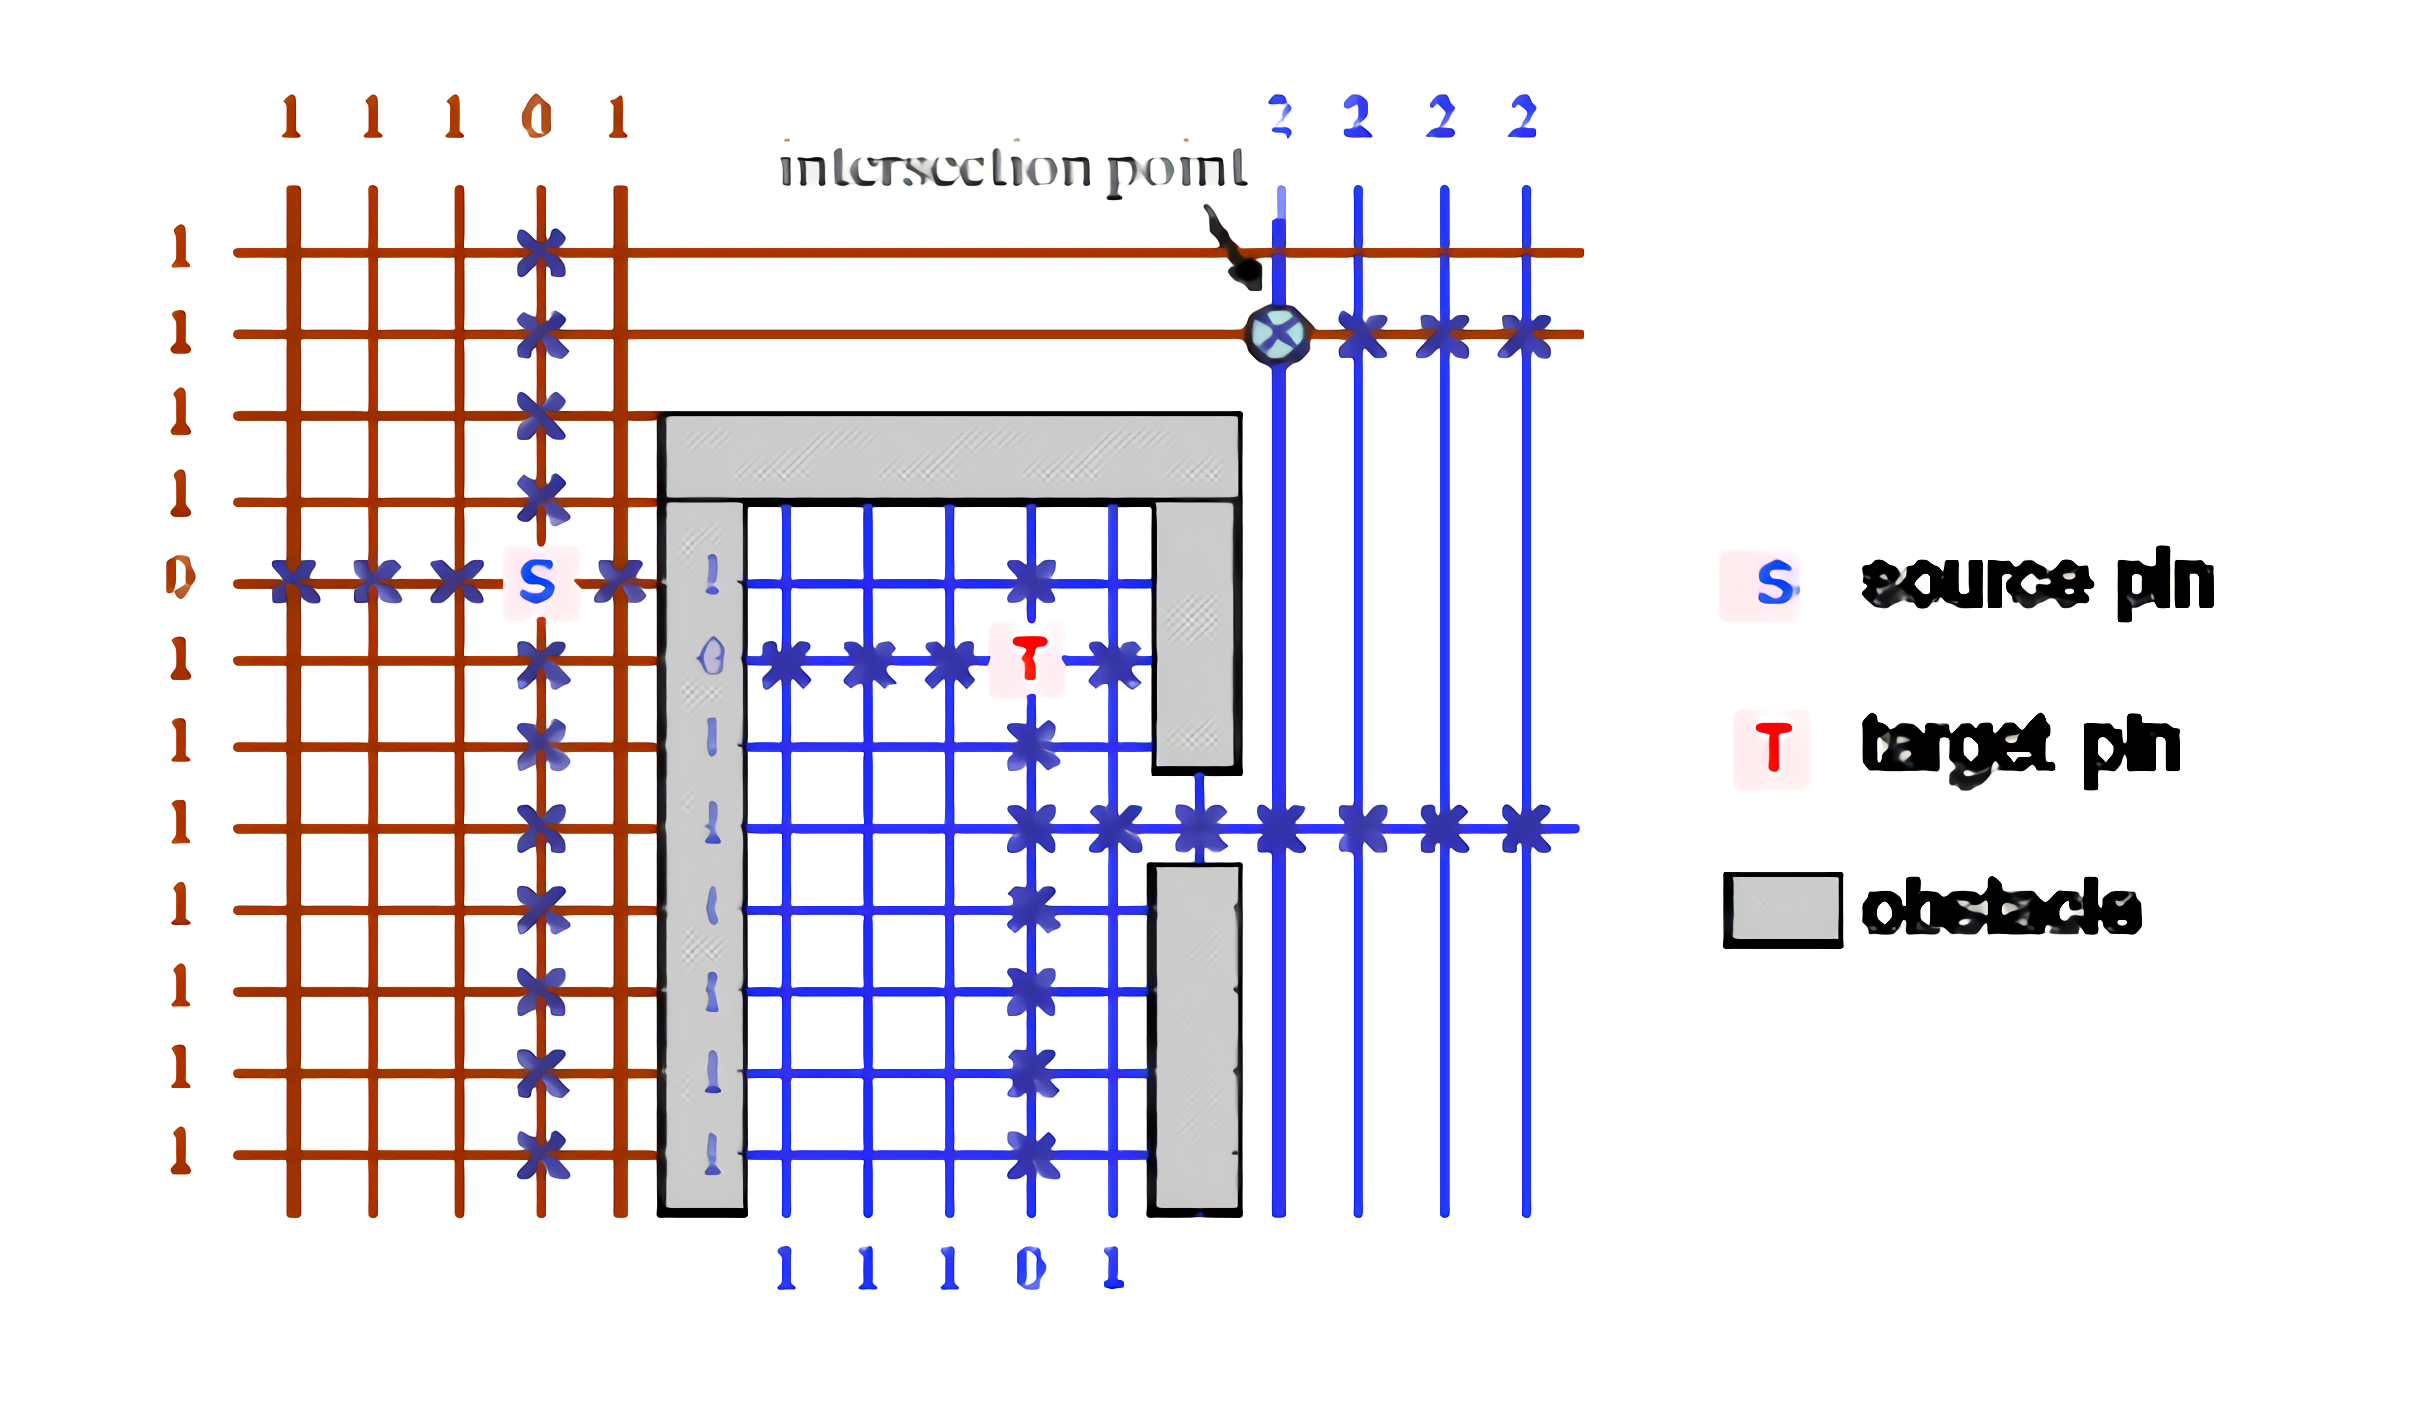
\includegraphics[width=\linewidth]{figures/mikami.png}
    \caption{Mikami Algorithm Illustration \cite{chen2009global}}
    \label{fig:mikamiIllustr}
\end{figure}

Mikami-Tabuchi algorithm wasn't designed with multilayer in mind. But it could be extended to work with multilayers by using 3d probes/lines and representing the VIAs as lines that's perpendicular to the layer. If a line in the layer intersected with the VIA line, the algorithm, recursively, extends a probe on the same point but on the other layer.

\begin{algorithm}[]
\SetAlgoLined
\KwResult{Some path between source and destination.}
    Let S and T be a pair source and destination respectively\;
    Generate 4 lines (2 horizontal and 2 vertical) passing through S and T\;
    Extend these lines till they hit obstacles or the boundary of the layout\;
    \If{a line generated from S intersects a line generated from T}{
        backtrack to find path\;
        return path\;
    }
    $i \leftarrow 1$\;
    \While{no new lines were created}{
        \ForEach{line L $\in$ level $i-1$}{%
            \ForEach{Point p $\in$ line L}{%
                Generate a perpendicular line L2\;
                Extend line L2 till it hit obstacles or the boundary of the layout or intersects with other line L3, where $L3 \in level j$ and $j > 0$\;
                \If{L2 intersects with L3 and L2 and L3 are from different terminals}{%
                    backtrack to find path\;
                    return path\;
                }
            }
        }
        $i \leftarrow i+1$
    }
    \caption{Mikami-Tabuchi Algorithm for Automatic Routing \cite{mikamiPresent}}
\end{algorithm}